\documentclass[12pt,a4paper,oneside]{article}
\usepackage[top=2cm, bottom=2cm, left=1.5cm, right=1.5cm] {geometry}
\usepackage{amsmath, amssymb, fancyhdr}
\usepackage{tkz-euclide,tikz-3dplot, tikz,tkz-tab}
\usepackage[dethi]{ex_test}%dethi,loigiai,color,solcolor,book
\usetikzlibrary{shapes.geometric,arrows,decorations.pathmorphing,calc,intersections,angles}
%\usetkzobj{all}
\usepackage{pgfplots}
\usepgfplotslibrary{fillbetween}
\pgfplotsset{compat=1.9}
\usepackage[hidelinks,unicode]{hyperref}
\usepackage{esvect}
\def\vec{\vv}
\def\overrightarrow{\vv}
\newcommand{\hoac}[1]{ 
\left[\begin{aligned}#1\end{aligned}\right.}
\newcommand{\heva}[1]{
\left\{\begin{aligned}#1\end{aligned}\right.}
\renewcommand{\baselinestretch}{1.2}
\renewtheorem{ex}{\color{red}Câu}
\begin{document}
	\OPTN{kindTF=t, kindSA=}
\def\SSS{}
%\begin{comment}
\Opensolutionfile{ansbook}[ans/ansbook]
\Opensolutionfile{ans}[ans/ans]
%-------------------------
\OPTN{kindDrag=1}
\begin{ex}
	\drag
	{$8$}
	[2]{$\sqrt{117}$}
	{$104$}
	[1]{$9$}
	Bạn Minh chơi xếp một kim tự tháp nhiều tầng từ những mảnh gỗ nhỏ hình hợp chữ nhật. Ở tầng dưới cùng, bạn Minh xếp $25$ mảnh gỗ. Mỗi tầng tiếp theo, Minh dùng ít hơn tầng trước $3$ mảnh gỗ. Đến tầng cuối cùng, bạn Minh chỉ dùng $1$ mảnh gỗ. Như vậy, chiếc kim tự tháp của bạn Minh hoàn thành có \drop tầng và bạn Minh phải dùng tất cả \drop mảnh gỗ.\\
	\textbf{\underline{Chú ý}}:\\
	Đây là kiểu câu hỏi ``\textbf{\textit{Kéo thả}}'' khi thi trên máy tính, thí sinh chọn các phương án cho trước để kéo và thả vào các chỗ trống nhằm thu được các khẳng định đúng.
	\loigiai{
		Số mảnh gỗ mà bạn Minh xếp các tầng của kim tự tháp lập thành một cấp số cộng $(u_n)$ với số hạng đầu $u_1=25$, số hạng cuối $u_n=1$ và công sai $d=-3$.\\
		Do đó, ta có số tầng của kim tự tháp bằng số phần tử của cấp số cộng: $n=\dfrac{u_n - u_1}{d}+1=9$ và tổng số mảnh gỗ mà bạn Minh đã dùng là
		\[ S_n=u_1+u_2+\dots+u_n=\dfrac{9 \cdot (u_1+u_9)}{2}=117. \]
	}
\end{ex}
\begin{ex}
	\immini[thm]{
		Diện tích miền phẳng $D$ (tô màu đậm) được giới hạn bởi đồ thị các hàm số $y=\sin x$, $y=\cos x$ và trục $Oy$ bằng
		\choice
		{$\sqrt{2}-1$}
		{$1$}
		{\True $\sqrt{2}+1$}
		{$\sqrt{2}$}
		}
	{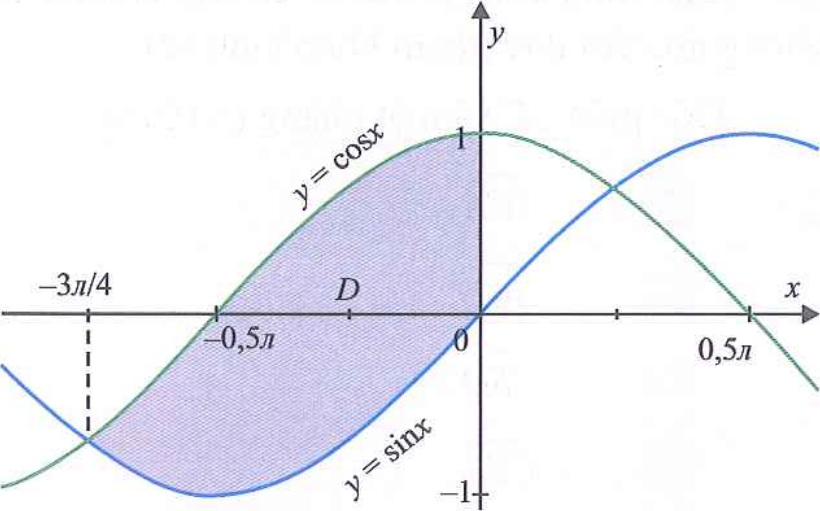
\includegraphics[width=0.4\linewidth] {Images/Cau2}}
	\loigiai{
		Từ hình vẽ, ta có:
		\[S(D)=\displaystyle\int\limits_{-\tfrac{3\pi}{4}}^{0} |\cos x - \sin x|\, \mathrm{\,d}x=\displaystyle\int\limits_{-\tfrac{3\pi}{4}}^{0} (\cos x - \sin x)\, \mathrm{\,d}x=(\sin x+\cos x)\bigg|_{-\tfrac{3\pi}{4}}^{0}=\sqrt{2}+1.\]
	}
\end{ex}

\begin{ex}
	Vũ và nhóm bạn lập kế hoạch đi tham quan lần lượt sáu địa điểm, ký hiệu là $A$, $B$, $C$, $D$, $E$, $F$. Mỗi lộ trình là một dãy có thứ tự các địa điểm này (mỗi địa điểm chỉ xuất hiện một lần). Có bao nhiêu cách chọn lộ trình tham quan, biết cả nhóm sẽ bắt đầu tham quan tại địa điểm $A$?
	\choice
	{$720$}
	{$3125$}
	{$15$}
	{\True $120$}
	\loigiai{
		Vì địa điểm bắt đầu tham quan của nhóm bạn cố định là $A$, nên mỗi lộ trình tham quan sẽ là một hoán vị của năm địa điểm còn lại.\\
		Do vậy, số cách chọn lộ trình tham quan là $P_5=5!=120$.
	}
\end{ex}

\begin{ex}
	\immini[thm]{
		Cho hình chóp $S.ABCD$ có đáy là hình vuông, $SA$ vuông góc với đáy (tham khảo hình vẽ). Góc giữa $SC$ và mặt phẳng $(SAD)$ là
		\choice
		{$\widehat{SCA}$}
		{$\widehat{SCD}$}
		{\True $\widehat{CSD}$}
		{$\widehat{CSA}$}
		}
	{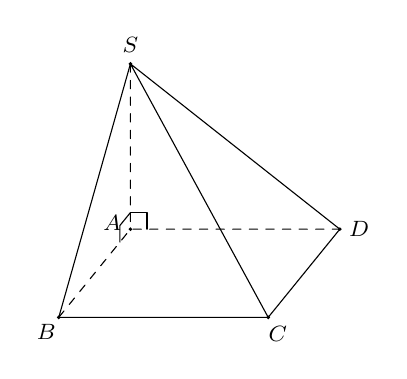
\begin{tikzpicture}[scale=0.7, font=\footnotesize, line join=round, line cap=round]
			\foreach \x\y\t in {0/3/S,0/0/A,-1.3/-1.6/B,2.5/-1.6/C}
			\coordinate (\t) at (\x,\y);
			\coordinate (D) at ($(A)+(C)-(B)$);
			\draw (S)--(C)--(B)--(S)--(D)--(C);
			\draw[dashed](S)--(A) (B)--(A)--(D);
			\path pic[draw,angle radius=6]{right angle=S--A--B}
			pic[draw,angle radius=6]{right angle=S--A--D};
			\foreach \t/\g in {S/90,A/160,B/-130,C/-60,D/0}
			\fill (\t) circle(1pt)
			node[shift={(\g:7pt)}]{$\t$};
		\end{tikzpicture}
	}
	\loigiai{
		Vì $SA \perp (ABCD)$ nên $SA \perp CD$.\\
		Mà $CD \perp AD$ nên $CD \perp (SAD)$.\\
		Do đó, $D$ là hình chiếu vuông góc của $C$ lên $(SAD)$.\\
		Bởi vậy, góc giữa $SC$ và mặt phẳng $(SAD)$ là $\widehat{CSD}$.
	}
\end{ex}

\begin{ex}
	Với các số thực dương $A$, $B$ bất kỳ, ta định nghĩa phép toán $A \uparrow B$ và $A \downarrow B$ như sau:
	\[ A \uparrow B=A^B \quad \text{và} \quad A \downarrow B=A^{-B}. \]
	Mỗi phát biểu sau đây là đúng hay sai?
	\choiceTF
	{$2 \uparrow 5=25$}
	{\True $4 \downarrow 3=\dfrac{1}{64}$}
	{\True Với mọi số nguyên dương $A, B, C$ thì $(2 \uparrow (A \downarrow B)) \uparrow C=2^{C \cdot A^{-B}}$}
	\loigiai{
		Ta có: $2 \uparrow 5=2^5=32$, $4 \downarrow 3=4^{-3}=\dfrac{1}{64}$.\\
		Với mọi số nguyên dương $A, B, C$ thì
		\[
		(2 \uparrow (A \downarrow B)) \uparrow C=(2 \uparrow (A^{-B})) \uparrow C=(2^{A^{-B}}) \uparrow C=(2^{A^{-B}})^C=2^{A^{-B}C}=2^{C \cdot A^{-B}}.
		\]
	}
\end{ex}

\begin{ex}
	Cho hàm số $y=f(x)$ xác định trên $\mathbb{R}\setminus\{1\}$ có bảng biến thiên như sau:
	\begin{center}
		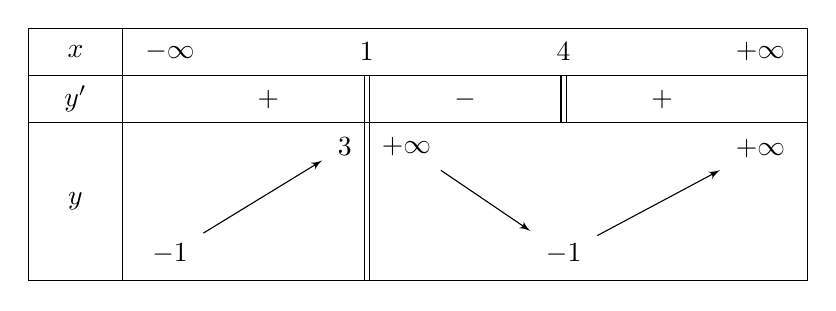
\begin{tikzpicture}
			\tikzset{double style/.append style={double distance=1.5pt}}
			\tkzTabInit[nocadre=false,lgt=1.2,espcl=2.5,deltacl=0.6]
			{$x$/0.6, $y'$/0.6, $y$/2}
			{$-\infty$,$1$,$4$,$+\infty$}
			\tkzTabLine{,+,d,-,d,+,}
			\tkzTabVar{-/$-1$,+D+/$3$/$+\infty$,-/$-1$,+/$+\infty$}
		\end{tikzpicture}
	\end{center}
	Mỗi phát biểu sau đây là đúng hay sai?
	\choiceTF
	{\True Hàm số $f(x)$ đạt cực tiểu tại $x=4$}
	{Hàm số $f(x)$ đạt cực đại tại $x=1$}
	{Hàm số $f(x)$ đạt cực tiểu tại $x=-1$}
	\loigiai{
		Từ bảng biến thiên, ta có:\\
		– Hàm số $f(x)$ đạt cực tiểu tại $x=4$, có giá trị cực tiểu là $y_{CT}=-1$. Do đó, phát biểu thứ nhất đúng.\\\
		– Vì hàm số $f(x)$ không xác định tại $x=1$ nên phát biểu thứ hai sai.\\
		– Dấu của $f'(x)$ không đổi khi $x$ đi qua $x_0=-1$, nên $x_0=-1$ không là điểm cực trị của $f(x)$. Do đó, phát biểu thứ ba sai.
	}
\end{ex}

\begin{ex}
	Cho hàm số $y=3+m\sin\left( 2x+\dfrac{\pi}{6} \right)$ với $m$ là tham số. Số giá trị nguyên của $m$ để giá trị lớn nhất của hàm số trên đoạn $\left[0; \dfrac{\pi}{2}\right]$ nhỏ hơn $10$ là 
	\shortans[........................]{$20$}
	\loigiai{
		Vì $x \in \left[0; \dfrac{\pi}{2}\right]$ nên $2x+\dfrac{\pi}{6} \in \left[\dfrac{\pi}{6}; \dfrac{7\pi}{6}\right]$. Do đó, $\sin \left(2x+\dfrac{\pi}{6}\right) \in \left[-\dfrac{1}{2};1\right]$.\\
		Xét hai trường hợp:\\
		TH1: Nếu $m \ge 0$ thì giá trị lớn nhất của hàm số trên $\left[0; \dfrac{\pi}{2}\right]$ là $\max\limits_{\left[0; \tfrac{\pi}{2}\right]} y=3+m$.\\
		Ta có $3+m<10 \Leftrightarrow m<7$. Bởi vậy, $m \in \{0; 1;\ldots; 6\}$ (có $7$ giá trị $m$).\\
		TH2: Nếu $m < 0$ thì giá trị lớn nhất của hàm số trên $\left[0; \dfrac{\pi}{2}\right]$ là $\max\limits_{\left[0; \tfrac{\pi}{2}\right]} y=3-\dfrac{m}{2}$.\\
		Ta có $3-\dfrac{m}{2}<10 \Leftrightarrow m>-14$.\\
		Bởi vậy, $m \in \{-13;-12;\ldots;-1\}$ (có $13$ giá trị $m$).\\
		Do đó, ta có tất cả $7+13=20$ giá trị của tham số $m$ thỏa mãn.
	}
\end{ex}

\begin{ex}
	Cho dãy số $(u_n)$ xác định bởi công thức $u_n=\dfrac{2n^2+1}{n+5}$ với $n \ge 1$. Mỗi phát biểu đây là đúng hay sai?
	\choiceTF
	{\True Dãy số $(u_n)$ là dãy tăng}
	{Dãy số $(u_n)$ bị chặn trên}
	\loigiai{
		Ta có $u_n=2n-10+\dfrac{51}{n+5}$.\\
		Do đó,
		$u_{n+1}-u_n=2+\dfrac{51}{n+6} - \dfrac{51}{n+5}=2-\dfrac{51}{(n+5)(n+6)} > 2-\dfrac{51}{5 \cdot 6} > 0$, 
		với mọi $n \ge 1$.\\
		Vì vậy, $u_{n+1} > u_n$ với mọi $n \ge 1$, dẫn đến dãy $(u_n)$ là dãy tăng.\\
		Mặt khác,
		\[ \lim u_n=\lim \dfrac{2n^2+1}{n+5}=\lim \dfrac{2n+\dfrac{1}{n}}{1+\dfrac{5}{n}}=+\infty \]
		nên dãy $(u_n)$ không bị chặn trên.
	}
\end{ex}

\begin{ex}
	\immini[thm]{
		Cho hàm số bậc bốn $y=f(x)$ có đồ thị của hàm số $y=f'(x)$ như hình vẽ. Những phát biểu nào dưới đây đúng?
		\choiceN
		{Hàm số $f(x)$ đồng biến trên $(0;2)$}
		{\True Hàm số $f(x)$ đồng biến trên các khoảng $(-\infty; a)$ và $(1;b)$}
		{Hàm số $f(x)$ nghịch biến trên $(-\infty;0)$}
		{\True Hàm số $f(x)$ nghịch biến trên $(0;1)$}}
	{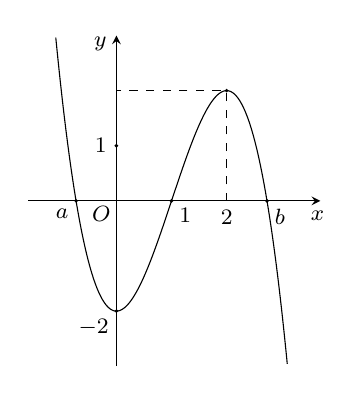
\begin{tikzpicture}[scale=0.7, font=\footnotesize, samples=200, >=stealth]
			\draw[->] (-1.6,0)--(3.7,0) node[below,xshift=-1]{$x$};
			\draw[->] (0,-3)--(0,3) node[left,yshift=-3]{$y$};
			\node at (0,0) [below left=-2pt]{$O$};
			\draw plot[domain=-1.1:3.1] (\x,{-(\x)^3+3*(\x)^2-2});
			\fill
			(0,-2) circle(1pt) node[below left=-1pt]{$-2$}
			(0,1) circle(1pt) node[left]{$1$}
			(1-sqrt 3,0) circle(1pt) node[below left=-1pt]{$a$}
			(1+sqrt 3,0) circle(1pt) node[below right=-1pt]{$b$}
			(1,0) circle(1pt) node[below right=-1pt]{$1$}
			(2,2) circle(1pt);
			\draw[dashed]
			(2,0) node[below]{$2$} |-(0,2);
	\end{tikzpicture}}
	\loigiai{
		Từ đồ thị của hàm số $y=f'(x)$, ta thấy:\\
		Trên các khoảng $(-\infty; a)$ và $(1; b)$, đồ thị hàm số $y=f'(x)$ nằm bên trên $Ox$ nên $f'(x)>0$ với mọi $x$ thuộc các khoảng này. Do đó, hàm số $f(x)$ đồng biến trên các khoảng này.\\
		Vậy phát biểu thứ hai đúng và phát biểu thứ ba sai.\\
		Trên các khoảng $(a; 1)$ và $(b; +\infty)$, đồ thị hàm số $y=f'(x)$ nằm bên dưới $Ox$ nên $f'(x)<0$ với mọi $x$ thuộc các khoảng này. Do đó, hàm số $f(x)$ nghịch biến trên các khoảng này.\\
		Hơn nữa, vì $(0; 1) \subset (a; 1)$ nên ta có $f(x)$ nghịch biến trên $(0; 1)$.\\
		Bởi vậy, phát biểu thứ tư đúng và phát biểu thứ nhất sai (vì $(0; 1) \subset (0; 2)$).
	}
\end{ex}

\begin{ex}
	Trong mặt phẳng $Oxy$, phương trình tiếp tuyến của đường tròn $(C)\colon x^2+y^2 - 2x+4y - 20=0$ tại $M(4;2)$ là
	\choice
	{\True $3x+4y-20=0$}
	{$y=2$}
	{$x=4$}
	{$4x+3y-22=0$}
	\loigiai{
		Đường tròn $(C)\colon (x-1)^2+(y+2)^2=25$ có tâm $I(1;-2)$.\\
		Đường thẳng $d$ tiếp xúc với $(C)$ tại điểm $M(4;2)$ nên $d \perp IM$, vì vậy $\vec{IM}=(3;4)$ là một vécto pháp tuyến của $d$.\\
		Phương trình của $d$ là
		$3(x-4)+4(y-2)=0 \Leftrightarrow 3x+4y-20=0$.
	}
\end{ex}

\begin{ex}
	Một robot đi từ điểm $A$ trên một đoạn đường thẳng, hướng về phía trước. Biết rằng mỗi lần bước, robot đó bước được $40$ cm hoặc $80$ cm. Với mỗi số nguyên dương $n$, gọi $a_n$ là tổng số cách robot đó di chuyển được quãng đường dài $40n$ (cm).\\
	Mỗi phát biểu sau đây là đúng hay sai?
	\choiceTF
	{\True $a_1=1$, $a_2=2$}
	{$a_{10} > a_9+a_8$}
	{\True $a_{10}=89$}
	{Nếu $a_n=233$ thì $n=13$}
	\loigiai{
		Gọi $B_n$ là điểm nằm trên đường đi của robot sao cho $AB_n=40n$ (cm).\\
		Với $n=1$, ta có $AB_1=40$ cm, nên chỉ có duy nhất một cách để robot di chuyển từ $A$ đến $B_1$ là bước một bước 40 cm. Do đó, $a_1=1$.\\
		Với $n=2$, ta có $AB_2=80$ cm, nên chỉ có hai cách để robot di chuyển từ $A$ đến $B_2$ là: bước hai bước 40 cm hoặc bước một bước 80 cm. Do đó, $a_2=2$.\\
		Với $n>2$, ta có $AB_n=40n$ cm. Để đến được $B_n$, robot đó có thể thực hiện theo hai phương án sau:\\
		Phương án 1: Di chuyển từ $A$ đến điểm $B_{n-2}$, cách $B_n$ một khoảng 80 cm, sau đó thực hiện một bước 80 cm. Số cách di chuyển của phương án này là $a_{n-2}$.\\
		Phương án 2: Di chuyển từ $A$ đến điểm $B_{n-1}$, cách $B_n$ một khoảng 40 cm, sau đó thực hiện một bước 40 cm. Số cách di chuyển của phương án này là $a_{n-1}$.\\
		Bởi vậy, ta có công thức truy hồi sau: $a_n=a_{n-1}+a_{n-2}$ với mọi $n>2$.\\
		Ta có bảng sau:
		\[
		\begin{tabular}{|c|c|c|c|c|c|c|c|c|c|c|c|c|c|}
			\hline
			$n$ & 1 & 2 & 3 & 4 & 5 & 6 & 7 & 8 & 9 & 10 & 11 & 12 & 13 \\
			\hline
			$a_n$ & 1 & 2 & 3 & 5 & 8 & 13 & 21 & 34 & 55 & 89 & 144 & 233 & 377 \\
			\hline
		\end{tabular}
		\]
		Từ bảng ta có $a_{10}=89$ và nếu $a_n=233$ thì $n=12$.
	}
\end{ex}

\begin{ex}
	Điền một số nguyên dương thích hợp vào chỗ trống.\\
	Cho hai hàm số $f(x)=\dfrac{25x}{x^2+1}$ và $g(x)=\dfrac{25x^3}{x^2+1}$. Khi đó, nếu $f'(x_0)=12$ thì $g'(x_0)=$%
	\shortans[..................]{$13$}
	\loigiai{
		Ta có $f'(x)=\dfrac{25(1-x^2)}{(x^2+1)^2}$, $f'(x)=12 \Leftrightarrow 12x^4+49x^2-13=0 \Leftrightarrow \begin{cases} x^2=\dfrac{1}{4} \\ x^2=\dfrac{-13}{3}. \end{cases}$\\
		Do đó, $x_0^2=\dfrac{1}{4}$.\\
		Vì $g'(x)=\dfrac{25x^2(x^2+3)}{(x^2+1)^2}$ nên $g'(x_0)=\dfrac{25x_0^2(x_0^2+3)}{(x_0^2+1)^2}=13$.
	}
\end{ex}

\begin{ex}
	Biết giới hạn $\lim\limits_{x \to \sqrt{3}} \dfrac{2x^2 - 6}{x - \sqrt{3}}=a\sqrt{b}$, trong đó $a$ là số nguyên và $b$ là số nguyên tố. Giá trị của biểu thức $P=a^2+b^2$ là
	\choice
	{$7$}
	{$19$}
	{\True $25$}
	{$13$}
	\loigiai{
		Ta có
		\[ \lim_{x \to \sqrt{3}} \dfrac{2x^2 - 6}{x - \sqrt{3}}=\lim_{x \to \sqrt{3}} \dfrac{2(x^2 - 3)}{x - \sqrt{3}}=\lim_{x \to \sqrt{3}} \dfrac{2(x - \sqrt{3})(x+\sqrt{3})}{x - \sqrt{3}}=\lim_{x \to \sqrt{3}} 2(x+\sqrt{3})=4\sqrt{3}.\]
		Do đó, $a=4$, $b=3$ và $P=25$.
	}
\end{ex}

\begin{ex}
	Có bao nhiêu giá trị nguyên của tham số $m$ thuộc đoạn $[-100;100]$ để hàm số
	$y=\dfrac{2^x+16}{2^x-m}$ nghịch biến trên $(1;5)$?
	\choice
	{$85$}
	{\True $87$}
	{$88$}
	{$116$}
	\loigiai{
		Ta có $y'=\dfrac{(-m-16)2^x \ln 2}{(2^x-m)^2}$. Nếu $y'=0$ thì $m=-16$. Khi đó $y=1$, là một hàm hằng.\\
		Bởi vậy, hàm số nghịch biến trên $(1;5)$ khi và chỉ khi $y'<0$ với mọi $x \in (1;5)$. Điều này tương đương với
		\[
		\begin{cases}
			m \ne 2^x \quad \forall x \in (1;5) \\
			-m-16 < 0
		\end{cases}
		\Leftrightarrow
		\begin{cases}
			m \notin (2;32) \\
			m > -16
		\end{cases}
		\]
		Kết hợp với $m \in [-100;100]$, ta được
		\[
		\begin{cases}
			-16 < m \le 2 \\
			32 \le m \le 100
		\end{cases}
		\]
		Có $18$ số nguyên thuộc $(-16;2]$ và có $69$ số nguyên thuộc $[32;100]$. Bởi vậy, ta có tất cả $18+69=87$ giá trị nguyên của $m$ thỏa mãn.
	}
\end{ex}

\begin{ex}
	\textit{Điền một số thích hợp vào chỗ trống}
	\begin{center}
		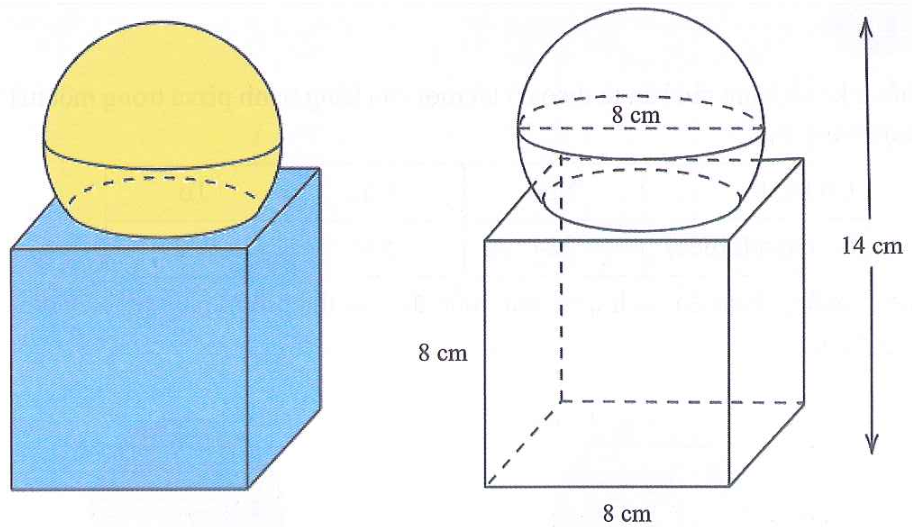
\includegraphics[width=0.8\linewidth] {Images/Cau15}
	\end{center}
	Một đồ lưu niệm bằng thủy tinh, có phần dưới là một khối lập phương và phần trên là một phần khối cầu. Biết đồ lưu niệm đó cao $14 \text{ cm}$; độ dài cạnh của khối lập phương và đường kính của khối cầu đều bằng $8 \text{ cm}$. Thể tích của đồ lưu niệm đó bằng \shortans[...............]{$738$}
	$\text{cm}^3$ (làm tròn kết quả đến hàng đơn vị).
	\loigiai{
		Thể tích của khối lập phương là $V_{\text{lp}}=8^3=512 \text{ (cm}^3)$.
		\begin{center}
			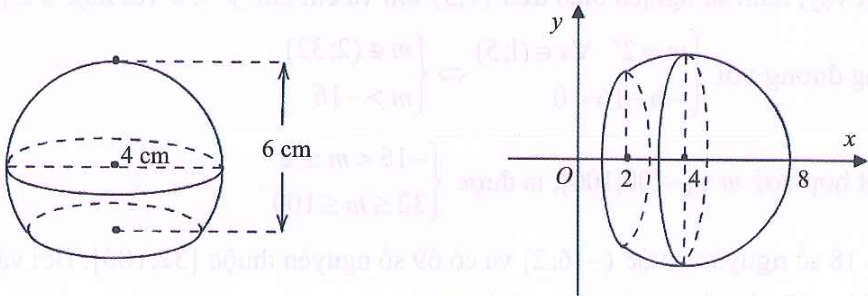
\includegraphics[width=0.8\linewidth] {Images/Cau15-2}
		\end{center}
		Mặt khác, ta thấy phần khối cầu có bán kính $4$ cm và chiều cao $14 - 8=6$ cm, sinh ra khi quay hình phẳng giới hạn bởi cung tròn có phương trình $y=\sqrt{8x - x^2}$, trục hoành $Ox$ và các đường thẳng $x=2$, $x=8$.\\
		Bởi vậy, thể tích phần khối cầu là
		\[ V_c=\pi \displaystyle\int\limits_2^8 (\sqrt{8x - x^2})^2 \mathrm{\,d}x=\pi \displaystyle\int\limits_2^8 (8x - x^2) \mathrm{\,d}x=72\pi \text{ (cm}^3\text{)}. \]
		Thể tích của đồ lưu niệm là
		\[ V=V_{tp}+V_c=512+72\pi \approx 738 \text{ (cm}^3\text{)}. \]
	}
\end{ex}

\begin{ex}
	Thống kê số bánh rán bán ra theo cỡ tại một cửa hàng bánh pizza trong một tuần, người ta thu được bảng sau:
	\[
	\begin{tabular}{|l|c|c|c|}
		\hline
		Cỡ bánh & Nhỏ & Vừa & To \\
		\hline
		Số bánh (chiếc) & 234 & 512 & 220 \\
		\hline
	\end{tabular}
	\]
	Trong những biểu đồ hình quạt sau, biểu đồ nào thích hợp nhất để biểu diễn dữ liệu trong bảng trên?
	\def\dotEX{}
	\choice
	{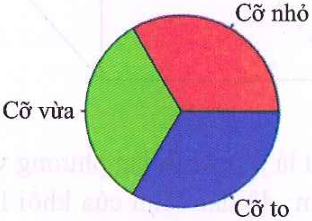
\includegraphics[width=0.42\linewidth] {Images/Cau16-1}}
	{\True 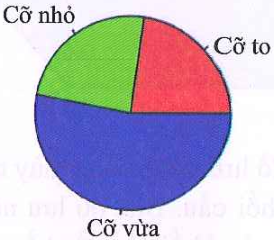
\includegraphics[width=0.42\linewidth] {Images/Cau16-2}}
	{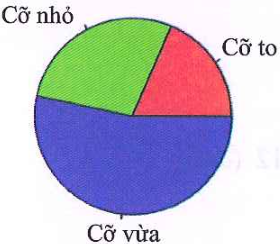
\includegraphics[width=0.42\linewidth] {Images/Cau16-3}}
	{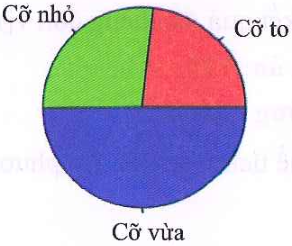
\includegraphics[width=0.42\linewidth] {Images/Cau16-4}}
	\loigiai{
		Tổng số bánh đã bán của cửa hàng trong tuần là $234+512+220=966$. Ta có bảng tần suất:
		\[
		\begin{tabular}{|l|c|c|c|}
			\hline
			Cỡ bánh & Nhỏ & Vừa & To \\
			\hline
			Số bánh (chiếc) & $234$ & $512$ & $220$ \\
			\hline
			Tần suất & $24\%$ & $53\%$ & $23\%$ \\
			\hline
		\end{tabular}
		\]
		Do đó, phần hình tròn biểu thị số bánh cỡ vừa chiếm hơn nửa hình tròn, các phần hình tròn biểu thị số bánh cỡ nhỏ và số bánh cỡ to xấp xỉ bằng nhau.
	}
\end{ex}

\begin{ex}
	Hàm số nào dưới đây là một nguyên hàm của hàm số $f(x)=2x+\sin 3x$ trên $\mathbb{R}$?
	\choice
	{$F(x)=x^2 - 3 \cos 3x$}
	{$G(x)=x^2 - \cos 3x+2$}
	{\True $H(x)=x^2 - \dfrac{\cos 3x}{3}$}
	{$R(x)=x^2+\dfrac{\cos 3x}{3}$}
	\loigiai{
		Ta có $F'(x)=2x+9 \sin 3x$, $G'(x)=2x+3 \sin 3x$, $H'(x)=2x+\sin 3x$,
		$R'(x)=2x - \sin 3x$.\\
		Do đó, $H'(x)=f(x) \forall x \in \mathbb{R}$.\\
		Vậy $H(x)$ là một nguyên hàm của $f(x)$ trên $\mathbb{R}$.
	}
\end{ex}

\begin{ex}
	\drag
	{$36$}
	[2]{$24$}
	[1]{$18$}
	{$30$}
	\immini{
	Cho hàm số $f(x)$ có đồ thị của hàm số $y=f'(x)$ trên đoạn $[0;10]$ như hình vẽ bên đây.\\
	Trên $[0;10]$ diện tích các hình phẳng giới hạn bởi đồ thị $y=f'(x)$ và trục $Ox$ lần lượt là $20, 6$ và $4$ (thể hiện như hình vẽ).\\
	Tích phân $\displaystyle\int\limits_{0}^{10} f'(x)\mathrm{\,d}x$ bằng \drop.\\
	Biết $f(0)=6$, giá trị của $f(10)$ bằng \drop.}
	{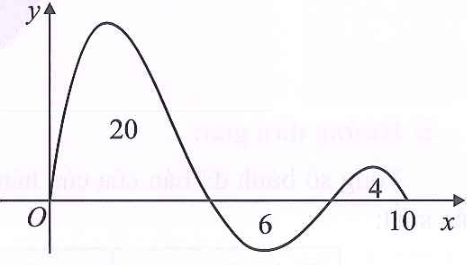
\includegraphics[width=0.4\linewidth] {Images/Cau18}}
	\loigiai{
		Gọi hoành độ các giao điểm còn lại của đồ thị và trục $Ox$ là $a$, $b$ ($a < b$). Khi đó, ta có
		\[
		\displaystyle\int\limits_0^{10} f'(x)\mathrm{\,d}x=\displaystyle\int\limits_0^a f'(x)\mathrm{\,d}x+\displaystyle\int\limits_a^b f'(x)\mathrm{\,d}x+\displaystyle\int\limits_b^{10} f'(x)\mathrm{\,d}x
		\]
		\[
		= \displaystyle\int\limits_0^a |f'(x)| \mathrm{\,d}x - \displaystyle\int\limits_a^b |f'(x)| \mathrm{\,d}x+\displaystyle\int\limits_b^{10} |f'(x)| \mathrm{\,d}x=20-6+4=18.
		\]
		Mặt khác,
		\[
		\displaystyle\int\limits_0^{10} f'(x)\mathrm{\,d}x=f(10) - f(0) \Rightarrow f(10)=\displaystyle\int\limits_0^{10} f'(x)\mathrm{\,d}x+f(0)=18+6=24.
		\]
	}
\end{ex}

\begin{ex}
	Điền một số tự nhiên thích hợp vào chỗ trống.
	Có hai thùng nước hình hộp chữ nhật, một thùng chứa đầy nước, thùng còn lại rỗng.
	Khi đặt cạnh nhau trên bàn như hình vẽ thì chúng tạo thành một khối lập phương cạnh bằng $1 \text{ (m)}$. Đổ một phần nước trong bình chứa đầy nước sang thùng không có nước, biết rằng trong quá trình đổ, nước không bị tràn ra ngoài; người ta quan sát thấy lượng nước của thùng ban đầu còn lại $\dfrac{3}{4}$ thùng và thùng kia chứa $\dfrac{1}{3}$ thùng.
	\begin{center}
		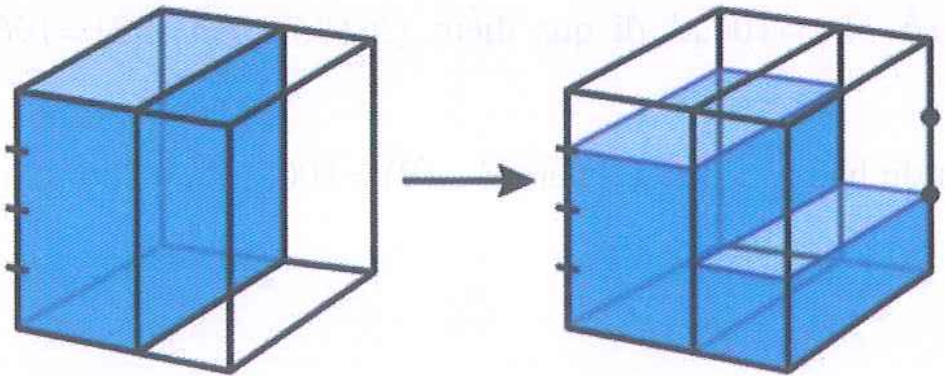
\includegraphics[width=0.8\linewidth]{Images/Cau19}
	\end{center}
	Thể tích thùng rỗng ban đầu là $\dfrac{a}{b}$ ($\text{m}^3$) với $a, b$ là các số nguyên dương và $\dfrac{a}{b}$ tối giản. 
	Giá trị của $a+b$ bằng %
	\shortans[.............]{$10$}
	\loigiai{
		Vì khi đặt cạnh nhau trên bàn, hai thùng nước tạo thành một khối lập phương cạnh
		bằng $1$ nên thể tích của thùng chứa đầy nước ban đầu là $1 - \dfrac{a}{b}$ ($\text{m}^3$). Sau khi đổ $1 - \dfrac{3}{4}=\dfrac{1}{4}$
		lượng nước của thùng chứa đầy nước sang cho thùng rỗng, thì thùng rỗng ban đầu chứa $\dfrac{1}{3}$
		thùng nên ta có $\dfrac{1}{4} \left(1 - \dfrac{a}{b}\right)=\dfrac{1}{3} \cdot \dfrac{a}{b}$. Từ đó tính được $\dfrac{a}{b}=\dfrac{3}{7}$. Do đó, $a+b=10$.
	}
\end{ex}

\begin{ex}
	Bác Việt mở một trang trại nuôi vịt. Trong 5 năm đầu, bác thống kê số lượng vịt phát triển được ghi lại như hình vẽ.
	\immini{
		Giả sử số lượng vịt (đơn vị: con) sau $t$ năm được tính theo hàm số $n(t)=100 \cdot a^{t}$ ($a$ là một hằng số và $t$ là số năm).\\
		Mỗi phát biểu sau đây là đúng hay sai?
		\choiceTF
		{Số lượng vịt ban đầu là $196$ con}
		{\True Dự báo số vit sau $9$ năm (đã làm tròn) là $2066$ con}}
	{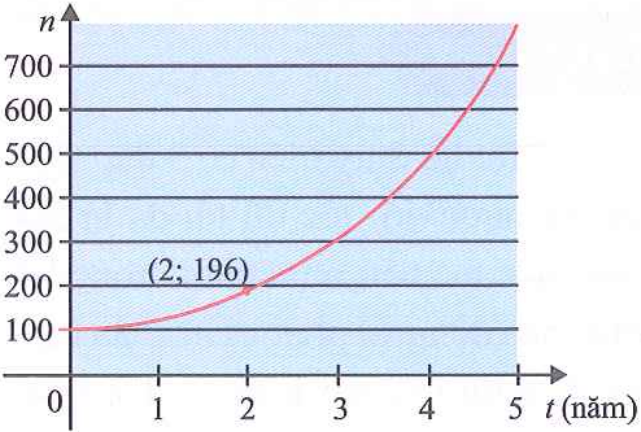
\includegraphics[width=0.4\linewidth] {Images/Cau20}}
	\loigiai{
		Quan sát đồ thị, ta thấy tại thời điểm ban đầu, tức là $t=0$, số vịt là $100$ con. Do đó,
		phát biểu thứ nhất là sai.\\
		Đồ thị hàm số $n(t)=100 \cdot a^t$ đi qua điểm $(2; 196)$ nên $n(2)=196 \Leftrightarrow 100 \cdot a^2=196$
		$\Rightarrow a=1.4$.
		Từ đó, suy ra dự báo số vịt sau 9 năm là $n(9)=100 \cdot 1.4^9 \approx 2066$ con.
	}
\end{ex}

\begin{ex}
	Trong không gian $Oxyz$, cho hình bình hành $ABCD$ có $A(3;-5;1)$, $B(-2;-1;4)$ và
	$C(7;-5;-2)$. Khi đó, tọa độ của điểm $D$ là
	\choice
	{\True $(12;-9;-5)$}
	{$(-6;-1;7)$}
	{$(2;-1;1)$}
	{$(8;-11;3)$}
	\loigiai{
		Gọi $D(a;b;c)$. Ta có $\vec{AB}=(-5;4;3)$ và $\vec{DC}=(7-a;-5-b;-2-c)$.\\
		Do $ABCD$ là hình bình hành nên $\vec{AB}=\vec{DC} \Leftrightarrow a=12; b=-9; c=-5$ hay $D(12;-9;-5)$.
	}
\end{ex}

\begin{ex}
	\immini[thm]{
		Một hồ thủy điện có $9$ đập tràn, mỗi đập có thể xả nước với tốc độ tối đa là $500$ $(\text{m}^3/\text{s})$. Do mưa liên tục nên mực nước trong hồ lên cao đến mức báo động và phải xả lũ khẩn cấp. Khi có lệnh xả lũ, người ta mở trước $5$ đập tràn và sau đó $5$ phút mở tiếp $4$ đập tràn còn lại. Biết rằng tốc độ lưu lượng nước qua mỗi đập tại thời điểm $t$ (giây) là $v(t)=k \cdot t$ $(\text{m}^3/\text{s})$ cho đến khi đạt tốc độ tối đa, trong đó $t$ là thời gian tính từ lúc đập đó được mở và $k$ là một hằng số. Giả sử sau $30$ phút từ khi có lệnh bắt đầu mở đập xả lũ, lưu lượng nước qua mỗi đập đều ở tốc độ tối đa và hồ thủy điện đã xả được $7387500$ $\text{m}^3$ nước. Khi đó, hằng số $k$ bằng
		\choice
		{$9$}
		{\True $10$}
		{$12$}
		{$15$}}
	{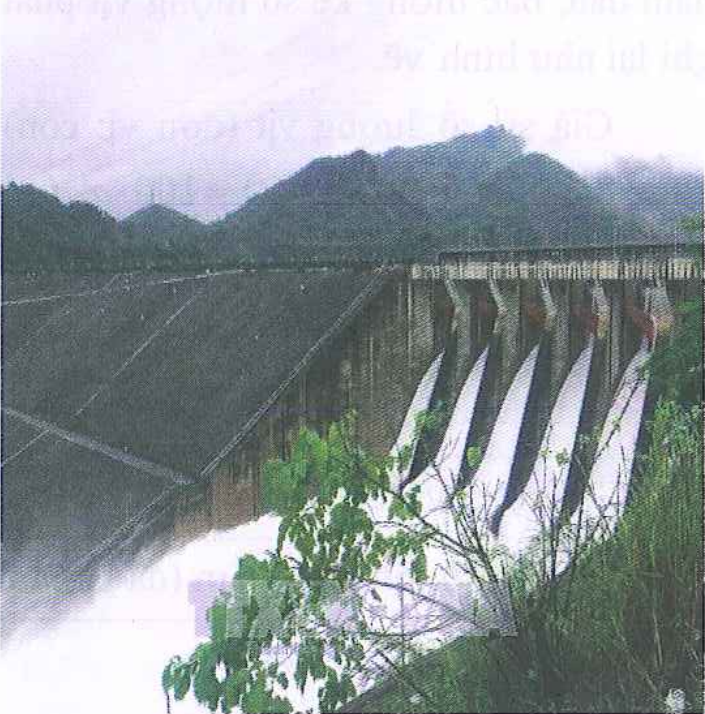
\includegraphics[width=0.4\linewidth] {Images/Cau22}}
	\loigiai{
		Lượng nước mà mỗi đập đã xả trong khoảng thời gian từ $a(s)$
		\[
		\Phi=\int_a^b v(t)dt.
		\]
		Vì tốc độ xả nước tối đa của mỗi đập là $500 \text{ m}^3/\text{s}$ nên thời gian tính từ khi mở đập xả lũ đến khi lưu lượng nước đạt tốc độ tối đa là: $t=t_0=\dfrac{500}{k}$ (giây). Do đó, công thức của $v(t)$ sẽ là
		\[
		v(t)=\begin{cases} kt & \text{khi } 0 \le t \le t_0 \\ 500 & \text{khi } t \ge t_0 \end{cases}
		\]
		Chú ý: 30 phút=1800 giây, 25 phút=1500 giây.\\
		Vì sau 30 phút từ khi có lệnh bắt đầu mở đập xả lũ, lưu lượng nước qua mỗi đập đều ở tốc độ tối đa nên:\\
		Trong 30 phút (1800 giây), lượng nước xả qua 5 đập được mở trước là
		\[
		\Phi_1=5 \cdot \int_{0}^{1800} v(t)dt=5 \left( \int_{0}^{t_0} ktdt+\int_{t_0}^{1800} 500dt \right) (\text{m}^3).
		\]
		Bốn đập thủy điện còn lại chỉ xả trong 25 phút (1500 giây). Lượng nước xả qua 4 đập
		còn lại là
		\[
		\Phi_2=4 \cdot \int_{0}^{1500} v(t)dt=4 \left( \int_{0}^{t_0} ktdt+\int_{t_0}^{1500} 500dt \right) (\text{m}^3).
		\]
		Hơn nữa, $kt_0=500$. Bởi vậy, lượng nước được xả qua 9 con đập sau 30 phút sẽ là
		\[
		\begin{aligned}
			\Phi_1+\Phi_2 &= 5 \left( \int_{0}^{t_0} ktdt+\int_{t_0}^{1800} 500dt \right)+4 \left( \int_{0}^{t_0} ktdt+\int_{t_0}^{1500} 500dt \right) \\
			&= \dfrac{9kt_0^2}{2} - 4500t_0+7500000=-2250t_0+7500000.
		\end{aligned}
		\]
		Ta có
		\[ -2250t_0+7500000=7387500 \Leftrightarrow t_0=50. \]
		Vậy
		\[ k=\dfrac{500}{t_0}=10. \]
	}
\end{ex}

\begin{ex}
	Tập xác định của hàm số $y=\log_2 (x-3)^2+\log_3 (x-1)$ là
	\choice
	{\True $D=(1;3) \cup (3;+\infty)$}
	{$D=(1;+\infty)$}
	{$D=(3;+\infty)$}
	{$D=[3;+\infty)$}
	\loigiai{
		Điều kiện xác định của hàm số là
		\[
		\begin{cases}
			(x-3)^2 > 0 \\
			x-1 > 0
		\end{cases}
		\Leftrightarrow
		\begin{cases}
			x \neq 3 \\
			x > 1
		\end{cases}
		\]
		Vậy tập xác định là $D=(1;3) \cup (3;+\infty)$.
	}
\end{ex}

\begin{ex}
	\immini[thm]{
		Cho hình chóp $S.ABC$ có $SA$ vuông góc với đáy và $SA=2a$, tam giác
		$A, AC=4a, AB=3a$ (xem hình vẽ).
		Gọi $\alpha$ là góc giữa mặt phẳng $(SBC)$ và mặt phẳng $(ABC)$, giá trị của $\tan\alpha$ bằng
		\choice
		{$\dfrac{2}{3}$}
		{$\dfrac{6}{5}$}
		{$\dfrac{4}{5}$}
		{\True $\dfrac{5}{6}$}}
	{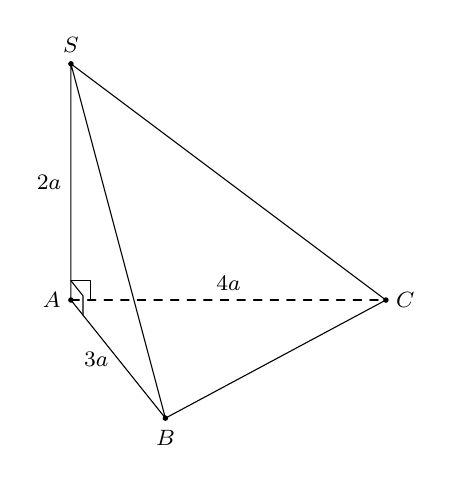
\begin{tikzpicture}[scale=1, font=\footnotesize, line join=round, line cap=round]
			\foreach \x\y\t in {0/3/S,0/0/A,1.2/-1.5/B,4/0/C}
			\coordinate (\t) at (\x,\y);
			\draw (S)--(B)--(A)--(S)--(C)--(B);
			\draw[dashed](A)--(C);
			\path pic[draw,angle radius=7]{right angle=S--A--B}
			pic[draw,angle radius=7]{right angle=S--A--C};
			\foreach \t/\g in {S/90,A/180,B/-90,C/0}
			\fill (\t) circle(1pt)
			node[shift={(\g:7pt)}]{$\t$};
			\path (A)--(B) node[pos=0.5,left]{$3a$};
			\path (A)--(C) node[pos=0.5,above]{$4a$};
			\path (A)--(S) node[pos=0.5,left]{$2a$};
		\end{tikzpicture}
	}
	\loigiai{
		\immini{
			Trong tam giác $ABC$ kẻ $AH \perp BC$. Mà $BC \perp SA$
			(do $SA \perp (ABC)$) nên $BC \perp (SAH)$. Vậy $\alpha=\widehat{SHA}$.
			Có $AH=\dfrac{AB \cdot AC}{BC}=\dfrac{12}{5}$, vậy $\tan \alpha=\dfrac{SA}{AH}=\dfrac{2}{\dfrac{12}{5}}=\dfrac{5}{6}$.}
		{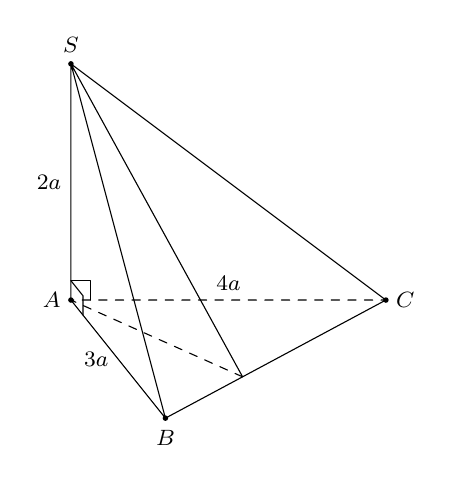
\begin{tikzpicture}[scale=1, font=\footnotesize, line join=round, line cap=round]
				\foreach \x\y\t in {0/3/S,0/0/A,1.2/-1.5/B,4/0/C}
				\coordinate (\t) at (\x,\y);
				\coordinate (H) at ($(B)!0.35!(C)$);
				\draw (H)--(S)--(B)--(A)--(S)--(C)--(B);
				\draw[dashed] (H)--(A)--(C);
				\path pic[draw,angle radius=7]{right angle=S--A--B}
				pic[draw,angle radius=7]{right angle=S--A--C};
				\foreach \t/\g in {S/90,A/180,B/-90,C/0}
				\fill (\t) circle(1pt)
				node[shift={(\g:7pt)}]{$\t$};
				\path (A)--(B) node[pos=0.5,left]{$3a$};
				\path (A)--(C) node[pos=0.5,above]{$4a$};
				\path (A)--(S) node[pos=0.5,left]{$2a$};
		\end{tikzpicture}}
	}
\end{ex}

\begin{ex}
	\numboxans{3}
	\drag
	[1]{$CE$}
	[2]{$DE$}
	[3]{đồng phẳng}
	{chéo nhau}
	[4]{$\dfrac{1}{3}$}
	{$\dfrac{2}{3}$}
	\textbf{Bài toán}: %
	Cho tứ diện $ABCD$. Gọi $I, J$ lần lượt là trọng tâm của tam giác $ABC$ và tam giác $ABD$. Chứng minh rằng $IJ \parallel CD$.\\
	\textbf{Lời giải}: %
	Gọi $E$ là trung điểm của $AB$. Ta có $I \in$ \drop, $J \in$ \drop nên $IJ$ và $CD$ \drop. Vì $I, J$ lần lượt là trọng tâm của tam giác $ABC$ và tam giác $ABD$ nên $\dfrac{EI}{EC}=\dfrac{EJ}{ED} =$ \drop.\\
	Theo định lý Thales đảo suy ra $IJ \parallel CD$ (đpcm).
	\loigiai{
		\immini{
			Gọi $E$ là trung điểm của $AB$. Ta có $I \in CE$, $J \in DE$ nên $IJ$ và $CD$ đồng phẳng. Vì $I, J$ lần lượt là trọng tâm của tam giác $ABC$ và tam giác $ABD$ nên
			\[ \dfrac{EI}{EC}=\dfrac{EJ}{ED}=\dfrac{1}{3}. \]
			Theo định lý Thales đảo suy ra $IJ // CD$ (đpcm).}
		{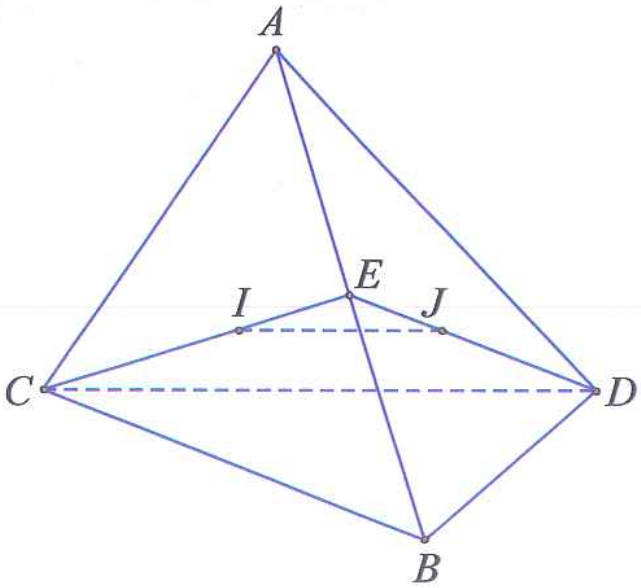
\includegraphics[width=0.4\linewidth] {Images/Cau25}}
	}
\end{ex}

\begin{ex}
	\textit{Điền một số thích hợp vào ô trống}
	\begin{center}
		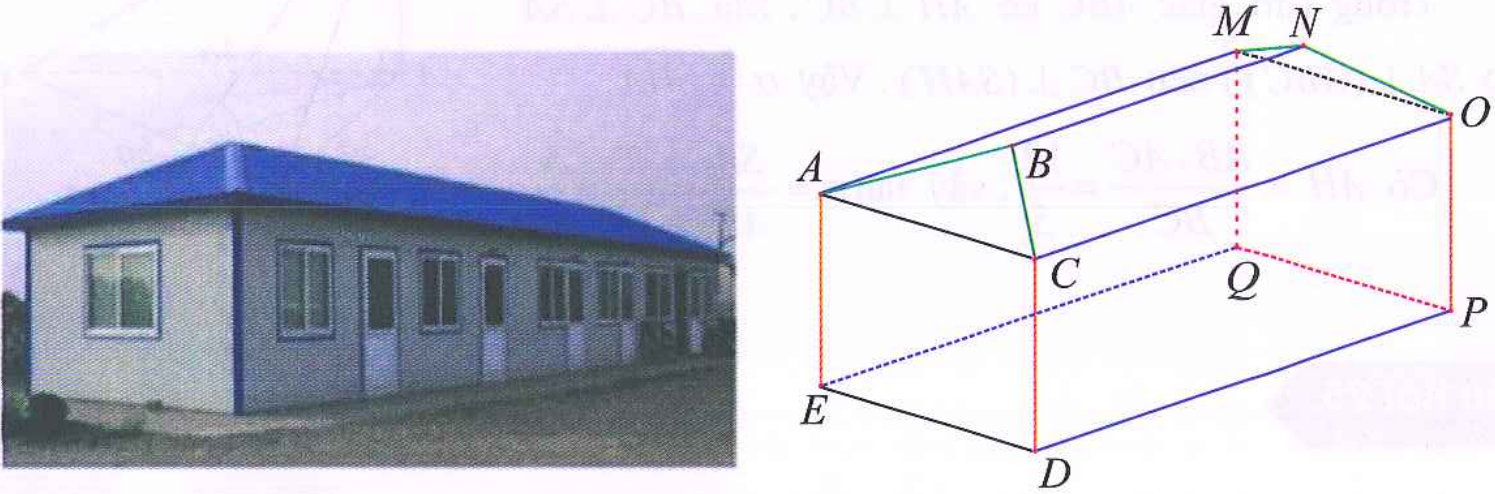
\includegraphics[width=0.8\linewidth] {Images/Cau26}
	\end{center}
	Giám đốc Long của một công ty xây dựng đang nghiên cứu xây nhà cho nhân viên của mình ở công trường. Ông Long tìm được một kiểu dáng ưng ý như hình ảnh. Ông vẽ lại khung nhà và đề xuất các thông số như sau: $ED=4(\text{m}), DP=16(\text{m}), CD=3(\text{m}), AB=BC=NO=MN=3(\text{m}), BN=12(\text{m}).$
	Tuy nhiên, ông Long nhớ ra rằng công trình có đường dây điện bên trên nên ông Long lo lắng về chiều cao của ngôi nhà (khoảng cách từ đường thẳng $BN$ đến mặt đất). Bằng tính toán, bạn hãy giúp ông Long biết chiều cao của ngôi nhà là bao nhiêu.
	Kết quả là: Nếu chiều cao của ngôi nhà là $h$ (m) thì $h^2=$%
	\shortans[.................]{$16$}
	\loigiai{
		\begin{center}
			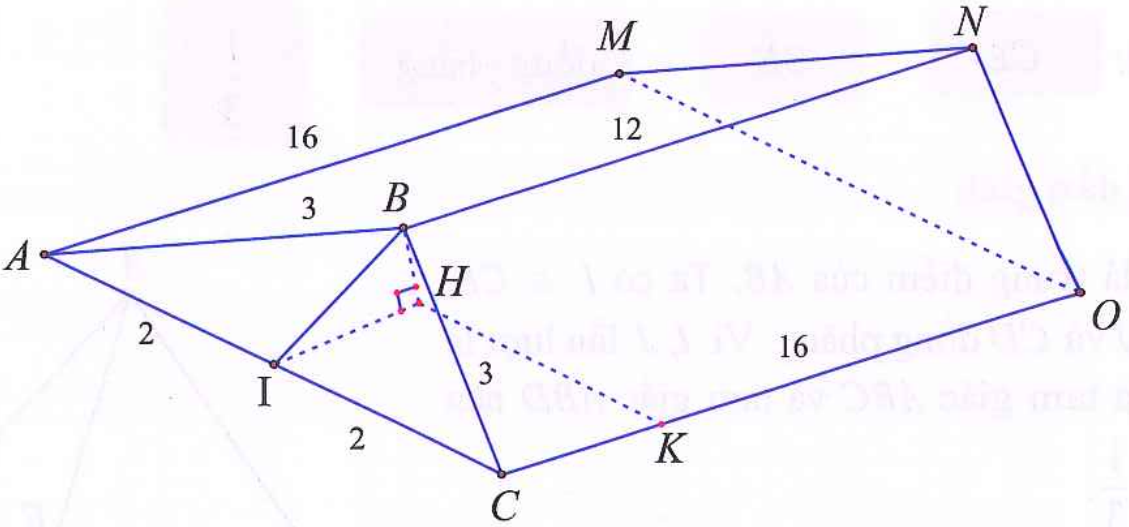
\includegraphics[width=0.8\linewidth] {Images/Cau26-2}
		\end{center}
		Vì hai mặt phẳng $(ACOM)$ và $(EDPQ)$ song song nên chiều cao của ngôi nhà sẽ là
		\[h=d(((EDPQ);(ACOM)))+d(B;(ACOM))=CD+d(B;(ACOM))=3+d(B;(ACOM)).\]
		Ta có $AC=ED=4$ (m), $AM=CO=DP=16$ (m).\\
		Gọi $I$ là trung điểm của $AC$, $H$ là hình chiếu vuông góc của $B$ lên mặt phẳng $(ACOM)$,
		$K$ là hình chiếu vuông góc của $H$ lên $CO$. Khi đó $AI=\dfrac{1}{2}AC=2$ (m). Hơn nữa, vì $AB=BC$
		nên tam giác $ABC$ là tam giác cân; dẫn đến $BI \perp AC$ và $BI^2=AB^2 - AI^2=5$ (m$^2$).\\
		Lại có $BH \perp AC$ (vì $BH \perp (ACOM)$) nên $AC \perp (BIH)$. Do đó, $AC \perp HI$. Bởi vậy,
		tứ giác $HKCI$ có ba góc vuông nên nó là hình chữ nhật. Mặt khác,
		$CK=IH=\dfrac{1}{2}(CO-BN)=2$ (m).\\
		Trong tam giác $BIH$, ta có $BH=\sqrt{BI^2 - IH^2}=\sqrt{5-4}=1$ (m). Vậy
		$d(B;(ACOM))=1$ (m) và chiều cao của ngôi nhà là $h=4$ (m). Bởi vậy, $h^2=16$.
	}
\end{ex}

\begin{ex}
	\textit{Điền một số nguyên thích hợp vào chỗ trống}.\\
	Một bác thợ định gò một chiếc thùng hình trụ bằng tôn không có nắp đậy để đựng nước. Biết thể tích nước đựng được là $8\pi$ (\text{dm}$^3$), độ dày của miếng tôn và mối hàn không đáng kể. Để tốn ít vật liệu nhất thì bác thợ cần làm chiếc thùng có chiều cao $h=a+b\pi$ (\text{dm}) với $a, b$ là các số nguyên. Khi đó, tổng $a^6+b^6$ bằng %
	\shortans[..............]{$64$}
	\loigiai{
		Gọi $R$ (\text{dm}) là bán kính của hình trụ. Khi đó, ta có $\pi R^2 h=8\pi$ (1).\\
		Vì chiếc thùng không có nắp và độ dày của các mối hàn không đáng kể nên diện tích tôn cần dùng để làm chiếc thùng là $S=S_{\text{xq}}+S_{\text{đ}}=2\pi Rh+\pi R^2$ (2).\\
		Từ (1) suy ra $Rh=\dfrac{8}{R}$, thế vào (2) ta được
		\[ S=\dfrac{16\pi}{R}+\pi R^2=\pi \left( \dfrac{8}{R}+\dfrac{8}{R}+R^2 \right) \geq 3\pi \sqrt[3]{\dfrac{8}{R} \cdot \dfrac{8}{R} \cdot R^2}=12\pi . \]
		Do đó, $\text{MinS}=12\pi$ đạt được khi $\dfrac{8}{R}=R^2 \Rightarrow R=2 \Rightarrow h=2$. Suy ra $a=2, b=0$.
		Vậy $a^6+b^6=64$.
	}
\end{ex}
%-------------------------
\Closesolutionfile{ans}
\Closesolutionfile{ansbook}
%\end{comment}
%===================
\begin{center}\bf\Large
	BẢNG ĐÁP ÁN
\end{center}
\inputansbox[0]{7}{ans/ans.tex}
%===================
%\begin{center}\bf\Large
%	LỜI GIẢI CHI TIẾT (tuỳ chọn [book])
%\end{center}
%\input{ans/ansbook.tex}
\end{document}
